\documentclass[dvipdfmx]{beamer}

\usepackage{beamerthemesplit}
\usepackage[]{graphicx}
\graphicspath{%
{./slide01-img/}%
{./text01-img/}%
}
% !TEX root = ./slide01-4.tex

\usepackage{listings}
\usepackage{hyperref}
\usepackage{pxjahyper}
\usepackage{color}

\setbeamertemplate{footline}[frame number]
\title{子どもIT未来塾 第1回}
\author{塾長 清水尚彦}

\def\quiz{1}

\begin{document}

\frame{
   \begin{center}
    \huge{子どもIT未来塾}\\

    \vspace{48pt}
	   \Large{第1回}\\
	   {\huge\bf ラズベリーパイの使い方・\\
	   \huge\bf 自己紹介ページを作ろう}\\
    \vspace{24pt}
    \large{塾長 清水尚彦}\\
    \vspace{10pt}
    \large{\the\year 年 6月24日}
  \end{center}
}



\begin{frame}[fragile]
	\frametitle{4時間目:自分のホームページを作ろう P.44-75~~~\raisebox{-3mm}{
\includegraphics[width=0.1\textwidth]{raspberry}}}
    \begin{figure}
      \centering
      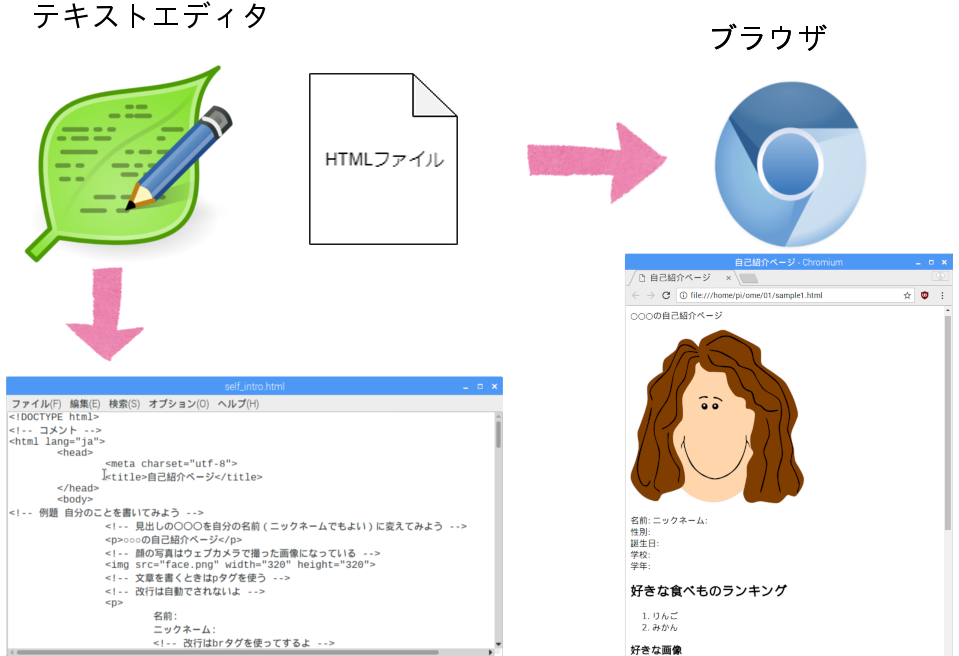
\includegraphics[width=0.7\textwidth]{slide04_001.png}\\
    \end{figure}
    \large\textbf{ホームページはHTMLという形式で書かれています}
        \begin{itemize}
          \item HTMLファイルをへんしゅうして、自分のホームページをつくろう
        \end{itemize}
\end{frame}

\begin{frame}[fragile]
	\frametitle{\large{HTMLファイルをブラウザで開いてみようP.45-47}~~~\raisebox{-3mm}{
\includegraphics[width=0.1\textwidth]{raspberry}}}
      \large\textbf{教科書をよみながら、じゅんばんに例題をやってみよう}
				\begin{itemize}
					\item 例題1-18 教材をじぶんのフォルダに置こう
					\item 例題1-19 ホームページの中身を見てみよう
				\end{itemize}
      \vfill
      \large\textbf{早く終わった子は、次の問題にチャレンジしよう}
      \begin{itemize}
        \item 問題1-17
      \end{itemize}
      \vfill
      \large\textbf{わからないことは、放っておかず、すぐに TA に聞きましょう}
\end{frame}

\begin{frame}[fragile]
	\frametitle{HTMLファイルをへんしゅうしてみようP.48-53~~~\raisebox{-3mm}{
\includegraphics[width=0.1\textwidth]{raspberry}}}
    \begin{minipage}[b]{0.47\textwidth}
      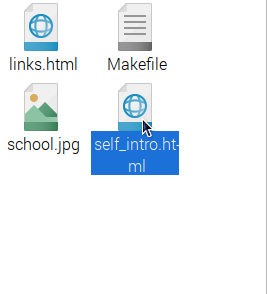
\includegraphics[width=\textwidth]{slide04_013.png}
      \begin{itemize}
        \item ブラウザで開くときはダブルクリック
      \end{itemize}
      \medskip
    \end{minipage}  
    \hfill    
    \begin{minipage}[b]{0.47\textwidth}
      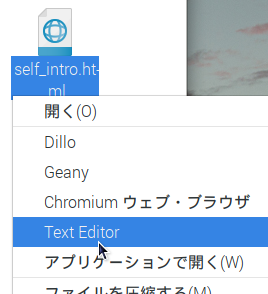
\includegraphics[width=\textwidth]{slide04_014.png}
      \begin{itemize}
        \item テキストエディタで開くときは、右クリックして出るメニューから開こう
      \end{itemize}
    \end{minipage} 
\end{frame}

\begin{frame}[fragile]
	\frametitle{HTMLファイルをへんしゅうしてみようP.48-53~~~\raisebox{-3mm}{
\includegraphics[width=0.1\textwidth]{raspberry}}}
    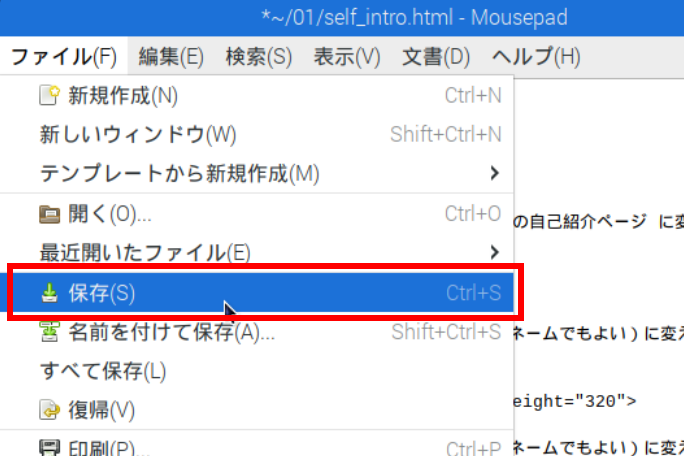
\includegraphics[width=0.5\textwidth]{slide04_003.png}
    \begin{minipage}[b]{0.05\textwidth}
    
\includegraphics[width=\textwidth]{slide04_005.png}
    \bigskip
    \end{minipage}
    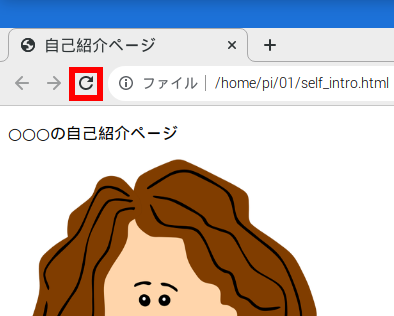
\includegraphics[width=0.41\textwidth]{slide04_004.png}
    \vfill
    \large\textbf{HTMLファイルをテキストエディタでへんしゅうしよう}
        \begin{itemize}
          \item ファイルをテキストエディタでへんしゅうしたら、保存をわすれないようにしましょう。
          \item 保存したら、ブラウザを更新しよう
        \end{itemize}
\end{frame}

\begin{frame}[fragile]
	\frametitle{HTMLファイルをへんしゅうしてみようP.48-53~~~\raisebox{-3mm}{
\includegraphics[width=0.1\textwidth]{raspberry}}}
      \large\textbf{教科書をよみながら、じゅんばんに例題をやってみよう}
				\begin{itemize}
					\item 例題1-20 ホームページの中身をのぞいてみよう
					\item 例題1-21 見出しを作ってみよう
				\end{itemize}
      \vfill
      \large\textbf{早く終わった子は、次の問題にチャレンジしよう}
      \begin{itemize}
        \item 問題1-18
      \end{itemize}
      \vfill
      \large\textbf{わからないことは、放っておかず、すぐに TA に聞きましょう}
\end{frame}

\begin{frame}[fragile]
	\frametitle{ホームページをつくってみようP.54-75~~~\raisebox{-3mm}{
\includegraphics[width=0.1\textwidth]{raspberry}}}
    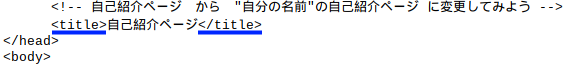
\includegraphics[width=0.8\textwidth]{slide04_006.png}
    \hfill
    
\includegraphics[width=0.1\textwidth]{slide04_008.png}
    \vfill
    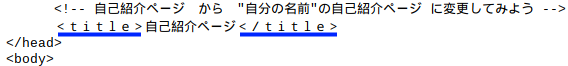
\includegraphics[width=0.8\textwidth]{slide04_007.png}
    \hfill
    
\includegraphics[width=0.1\textwidth]{slide04_009.png}
    \vfill
    \large\textbf{さまざまなタグを使ってホームページをつくります}
        \begin{itemize}
          \item タグは、必ず\textcolor[rgb]{1.0,0.2,0.2}{半角}で入力しよう(〇: 半角 ×: 全角)
          \item 24-25ページをみて、入力モードのきりかえかたを復習しよう
        \end{itemize}
\end{frame}

\begin{frame}[fragile]
	\frametitle{ホームページをつくってみようP.54-75~~~\raisebox{-3mm}{
\includegraphics[width=0.1\textwidth]{raspberry}}}
      \large\textbf{教科書をよみながら、じゅんばんに例題をやってみよう}
				\begin{itemize}
					\item 例題1-22 ホームページの中身をのぞいてみよう
					\item 例題1-23 自分のことを紹介しよう
					\item 例題1-24 ランキングを作ろう
					\item 例題1-25 日記を書いてみよう
					\item 例題1-26 グループのメンバー表を作ろう
					\item 例題1-27 自分の好きなホームページを紹介しよう
					\item 例題1-28 教室の使うものリストを作ろう
				\end{itemize}
      \vfill
      \large\textbf{早く終わった子は、次の問題にチャレンジしよう}
      \begin{itemize}
        \item 問題1-19~問題1-30、78ページのチャレンジ問題
      \end{itemize}
      \vfill
      \large\textbf{わからないことは、放っておかず、すぐに TA に聞きましょう}
\end{frame}

\begin{frame}[fragile]
	\frametitle{でんげんの切り方をおぼえようP.76-77~~~\raisebox{-3mm}{
\includegraphics[width=0.1\textwidth]{raspberry}}}
  \begin{figure}
    \centering
    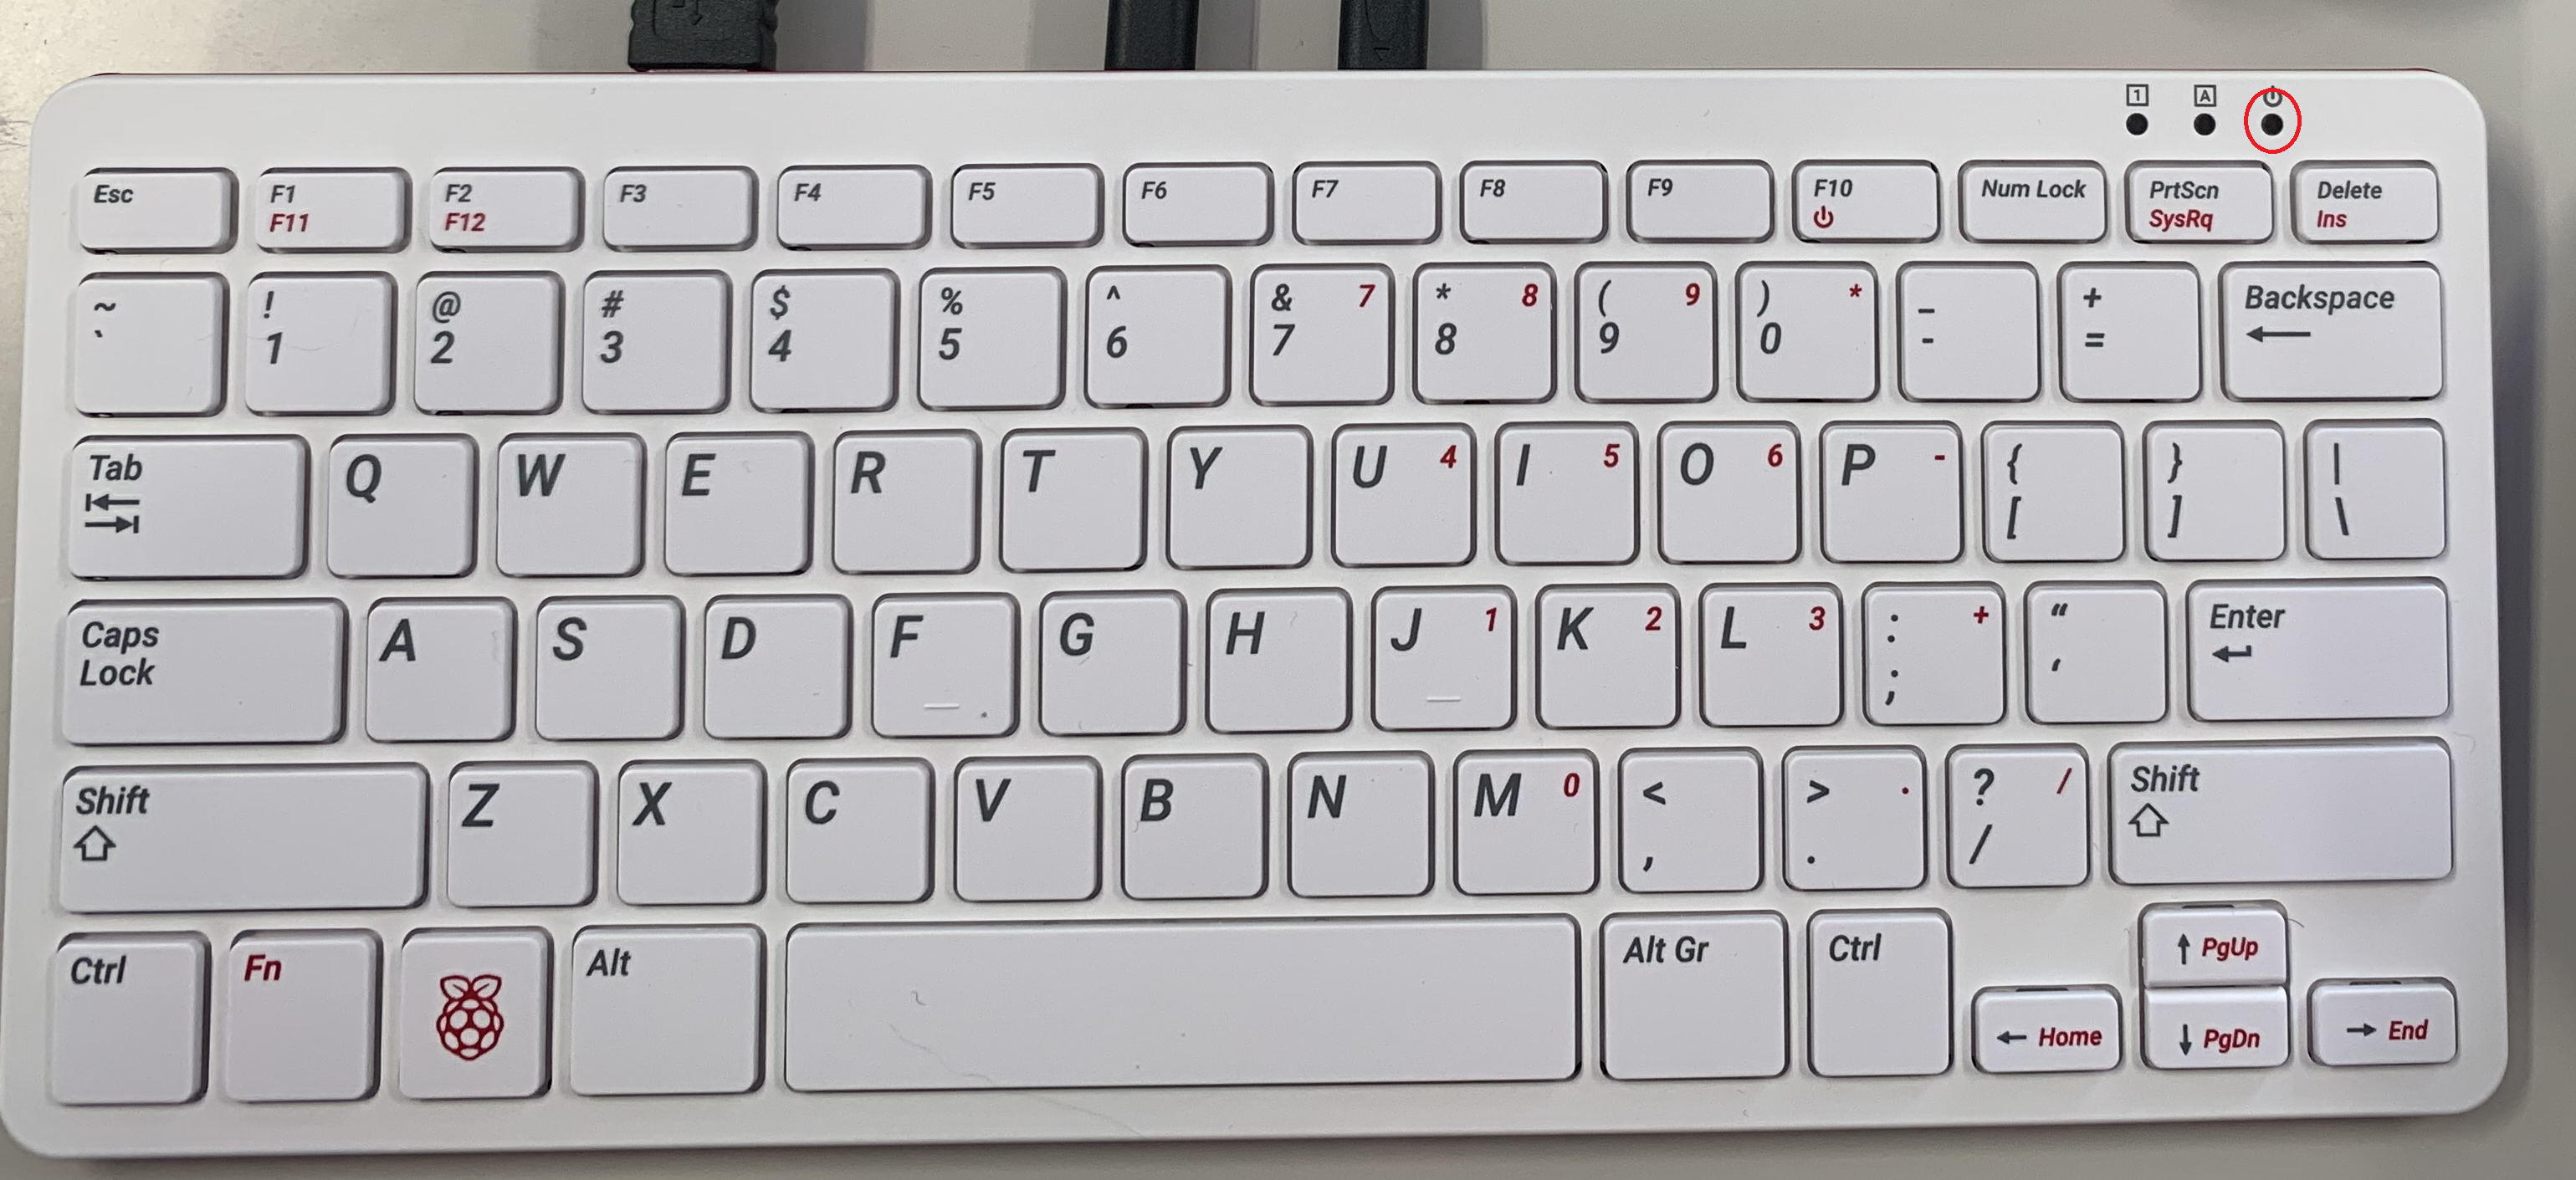
\includegraphics[width=0.7\textwidth]{slide04_010.png}
  \end{figure}
    \vfill
    \large\textbf{76ページを読んで、ラズベリーパイのでんげんを切ろう}
        \begin{itemize}
          \item 右上のでんげんランプが消えたことをかくにんしてから、でんげんアダプタをコンセントから抜きましょう
          \item \textcolor[rgb]{1.0,0.2,0.2}{ランプが消える前にアダプタを抜いてはいけません。microSDカードがこわれる可能性があります。}
        \end{itemize}
\end{frame}

\begin{frame}[fragile]
	\frametitle{お家でタイピングれんしゅうをしようP.28-30~~~\raisebox{-3mm}{
\includegraphics[width=0.1\textwidth]{raspberry}}}
    \begin{figure}
      \centering
      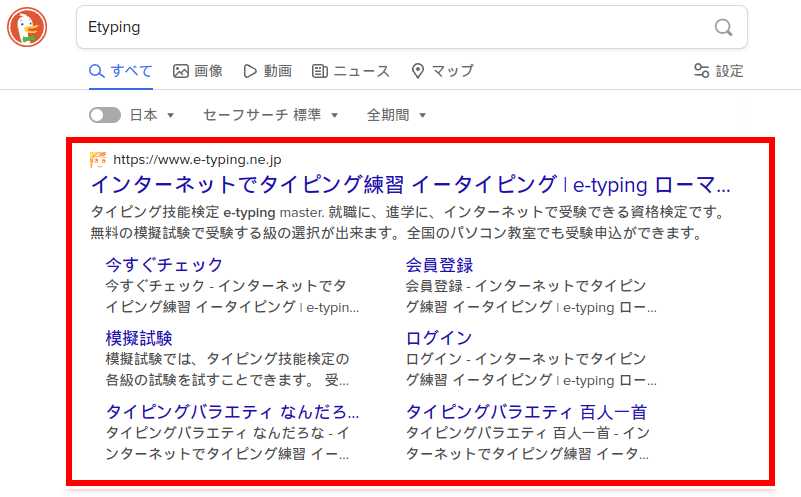
\includegraphics[width=0.7\textwidth]{slide04_015.png}
    \end{figure}
      \begin{itemize}
        \item タイピングがはやいと、プログラミングもやりやすくなるよ
        \item 練習すればだれでもはやくなります。28ページで紹介したサイトをつかって、お家で練習してみよう
        \item インターネット上にはさまざまなタイピングゲームがあります。けんさくして見つけた好きなゲームで練習してみよう
      \end{itemize}
\end{frame}

\begin{frame}[fragile]
	\frametitle{質問フォームP.90-92~~~\raisebox{-3mm}{
\includegraphics[width=0.1\textwidth]{raspberry}}}
    \begin{minipage}{0.6\textwidth}
      \begin{itemize}
        \item 今日できなかった問題は、家でやってみてね
        \bigskip
        \item 問題の解答例は79-90ページにあるよ
        \bigskip
        \item わからないことがあったら、質問フォームをつかって質問しよう
      \end{itemize}
      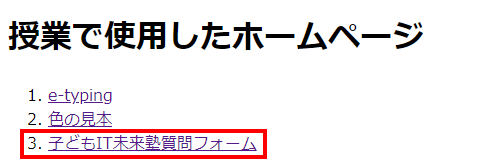
\includegraphics[width=\textwidth]{slide04_012.png}
    \end{minipage}    
    \hfill
    \begin{minipage}{0.38\textwidth}
      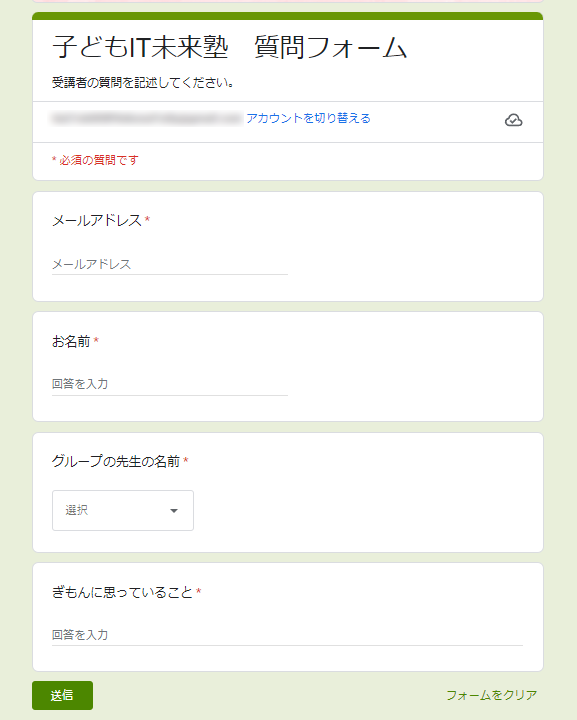
\includegraphics[height=0.7\textheight]{slide04_011.png}
    \end{minipage}
    \vfill
\end{frame}

\begin{frame}[fragile]
	\frametitle{おつかれさまでした!気を付けて帰ってください~~~\raisebox{-3mm}{
\includegraphics[width=0.1\textwidth]{raspberry}}}
     \large\textbf{注意点}
        \begin{itemize}
          \item ラズベリーパイなど電子機器はしんちょうに扱いましょう
          \bigskip
          \item ラズベリーパイは付属の箱にいれて持ち帰りましょう
          \bigskip
          \item microSDカードはラズベリーパイにさしたままにしておきましょう
          \bigskip
          \item わすれものの無いようにしましょう
        \end{itemize}
\end{frame}

\end{document}

